%% Preambulo general para documentos de apuntes y notas matematicas
\documentclass[12pt,letterpaper]{article}
% Paquetes para manejar idiomas != English
\usepackage[utf8]{inputenc}
\usepackage[T1]{fontenc}
\usepackage[english,spanish]{babel}
% Paquete para manejar referencias bibliogrfics
\usepackage{natbib}
% Paquete para manejar imagenes y graficos
\usepackage{graphicx}
% Paquete para manejar URLs
\usepackage{hyperref}
% Paquete para usar proposiciones condicionales
\usepackage{ifthen}
% Directorios para imagenes
% Ruta relativa
\graphicspath{
 {../../LaTeXyEclipse/img/}
 {../01A45Siglo17/01A45Img/}
 {../01A40Siglos15_16Renacimiento/01A40Img/} 
 }

\begin{document}
\title{Notas y apuntes sobre historia de las matem\'aticas}
\author{Jaime Gonz\'alez}
\date{Septiembre 2014}
\maketitle
\begin{abstract}
El presente documento presenta una serie de recursos elementales para el tema del mismo...

	\begin{center}
Clasificac\'on conforme a MSC 2010: 01-XX
	\end{center}

% Logo de LaTeX
	\begin{center}
		{\LaTeX}
	\end{center}
\end{abstract}

% Insertar figura
\begin{figure}[h!]
	\centering
		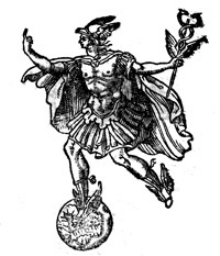
\includegraphics[scale=0.30]{MercurioBombelli.jpg}
		\caption{Mercurio, en el \'Algebra de Bombelli}
	\label{threadsVsSync}
	\end{figure}

\newpage
% Tablas de contenido
\tableofcontents
\listoffigures
%\listoftables

\newpage
% Primera secci\'on
\section{Definici\'on}
Cons\'ultese:
\href{http://www.math.niu.edu/~rusin/known-math/index/01-XX.html}{The Mathematical Atlas, 01 History and Biography}

\selectlanguage{english}
	\begin{quotation}
Formal studies in the history of mathematics developed much more slowly than
studies in mathematics itself. 
	\end{quotation}

\selectlanguage{spanish}

\subsection{F\'ormulas}
Ejemplos de f\'ormulas.

\begin{enumerate}
\item \label{set}
   $\left \{a , b \right \}$ es un conjunto
\item \label{gamma}
   $\Gamma\left(n\right)$ función gama
\item \label{isinteger}
   $n\choose r$ es un entero. 
\item \label{sum2n}
   ${n\choose 0}+{n\choose 1}+{n\choose 2}+\cdots+{n\choose n}=2^n$.
\item \label{sum0}
   ${n\choose 0}-{n\choose 1}+{n\choose 2}-\cdots+(-1)^n{n\choose n}=0$ for $n>0$.
\item \label{sump1}
   $\sum_{t=k}^n {t\choose k }={n+1\choose k+1}$.
\end{enumerate}

\section{Números triangulares}

$$f_{2}={{n\,\left(n+1\right)}\over{2}}$$

$$t={{n^2+n}\over{2}}$$

% Bibliograf
\citep{Edwards2002Pascals}

\citep{NIST:DLMF}

\bibliographystyle{plain}
% Ruta absoluta al archivo (sin espacios!)
%\bibliography{C:/Users/Milestone/Dropbox/Refer/Matemat/ApuntesRefsyRecursos/00MatematicasEnGeneral/00A15Bibliografia/00A15Bibliografia}
% Ruta relativa
\bibliography{../../00MatematicasEnGeneral/00A15Bibliografia/00A15Bibliografia}

\end{document}